% $Header: /cvsroot/latex-beamer/latex-beamer/solutions/generic-talks/generic-ornate-15min-45min.en.tex,v~1.5 2007/01/28 20:48:23 tantau Exp $

\documentclass{beamer}

% Copyright 2004 by Till Tantau <tantau@users.sourceforge.net>.
%
% In principle, this file can be redistributed and/or modified under
% the terms of the GNU Public License, version 2.
%
% However, this file is supposed to be a template to be modified
% for your own needs. For this reason, if you use this file as a
% template and not specifically distribute it as part of a another
% package/program, I grant the extra permission to freely copy and
% modify this file as you see fit and even to delete this copyright
% notice.

\def\Tiny{\fontsize{6pt}{6pt}\selectfont}
\def\supertiny{\fontsize{4pt}{4pt}\selectfont}

\mode<presentation>
{
  \usetheme{Warsaw}
  % \setbeamercovered{transparent}
  \usecolortheme{crane}
}


\usepackage{graphicx, ifthen, listings}

\usepackage[czech]{babel}
% \usefonttheme{professionalfonts}
\usepackage{times}
\usepackage{amsmath}
\usepackage[utf8]{inputenc}
\usepackage{wrapfig}

\usepackage[T1]{fontenc}

\lstset{ basicstyle=\tiny, stringstyle=\ttfamily, showstringspaces=false }

\everymath{\displaystyle}

\setbeamerfont{frametitle}{size=\large}
\setbeamerfont{subsection in toc}{size=\scriptsize}

\makeatletter\newenvironment{blackbox}{%
   \begin{lrbox}{\@tempboxa}\begin{minipage}{0.95\columnwidth}}{\end{minipage}\end{lrbox}%
   \colorbox{black}{\usebox{\@tempboxa}}
}\makeatother

\title[IMF (1)]{Informatika pro moderní fyziky (1)\\základy automatizace; jednoduché zpracování a vizualizace dat}

\author[Franti\v{s}ek HAVL\r{U}J, ORF ÚJV Řež]{Franti\v{s}ek HAVL\r{U}J\\{\scriptsize \emph{e-mail: haf@ujv.cz}}}

\date{semestr 2012/2013\\4. prosince 2012}

\institute[ORF ÚJV Řež]
{ÚJV Řež\\oddělení Reaktorové fyziky a podpory palivového cyklu}

\AtBeginSection[]
{
\begin{frame}<beamer>
\frametitle{Obsah}
\tableofcontents[currentsection,hideothersubsections]
\end{frame}
}

\begin{document}

\begin{frame}
  \titlepage
\end{frame}

\begin{frame}
  \tableofcontents
\end{frame}

\section{Úvod}

\subsection{K čemu je počítač?}

\begin{frame}{K čemu je počítač?}
  \begin{itemize}
    \item počítače udělají cokoliv, pokud na to existuje postup
    \item pokud na něco existuje postup, není na to potřeba člověk
    \item existuje-li proces, existuje také algoritmus
    \item kdo má algoritmus, může napsat program
  \end{itemize}
\end{frame}

\begin{frame}{Proč se zabývat automatizací?}
  \begin{itemize}
    \item mechanická práce je otravná
    \item program neudělá (náhodnou) chybu
    \item skript trvá stejně dlouho pro libovolný objem dat
    \item pokud je potřeba něco pozměnit nebo jen zpracování zopakovat, je ruční práce vepsí
  \end{itemize}
\end{frame}

\subsection{Problém č. 1: vykreslování dat z detektoru}

\begin{frame}{Zadání}
  \begin{block}{\# 1}
    Na konci provozní směny je potřeba vyhodnotit signály ze čtyř detektorů a vykreslit je do grafu (signál v závislosti na čase). Data dostáváte v jednoduchém textovém souboru (dva sloupce, spousta řádků). Je potřeba vykreslit do jednoho grafu všechny čtyři detektory. Potíž je, že taková data přicházejí každý den - tento úkol je tedy potřeba řešit opakovaně.
  \end{block}
  \begin{block}{S hvězdičkou}
    Počet detektorů je proměnný (1 až 9).
  \end{block}
\end{frame}

\subsection{Problém č. 2: mnoho výpočtů, inženýrova smrt}

\begin{frame}{Zadání}
  \begin{block}{\# 2}
    Při přípravě základního kritického experimentu je pomocí MCNP potřeba najít kritickou polohu regulační tyče R2. 
    
    Jak se tato poloha změní při změně polohy tyče R1?
  \end{block}
\end{frame}

\section{Ruční a poloautomatická řešení}

\subsection{Problém č. 1: rozbor situace}

\begin{frame}{Klasické řešení (MS Excel)}
  \begin{itemize}
    \item proveďte; jaké všechny kroky je potřeba udělat?
    \item na který z provedených kroků byl potřeba člověk -- co z toho by nemohl stejně dobře udělat počítač sám?
    \item jaké jsou výhody a nevýhody ručního řešení?
    \item jak by mělo takové automatické řešení fungovat?
  \end{itemize}
\end{frame}

\begin{frame}{Komponenty pro automatizaci}
  \begin{block}{Funkční části}
    výkonné programy (např. kreslení grafů, generování tabulek/reportů, spouštění výpočtů) -- předpokladem je možnost spouštět program v neinteraktivním (dávkovém) režimu
  \end{block}
  \begin{block}{Jak to slepit dohromady}
    dávkobý soubor (BAT) nebo skript -- je nutno vždy vhodně volit použité prostředky ve vztahu k jednoduchosti, požadavkům na funkce, přenositelnosti
  \end{block}
\end{frame}

\begin{frame}{Jak postupovat s automatickým řešením?}
  \begin{enumerate}
    \item vykreslit graf s jedním detektorem
    \pause
    \item se všemi detektory
    \pause
    \item z příkazové řádky
    \pause
    \item z batch souboru
    \pause
    \item se jménem adresáře jako parametrem
  \end{enumerate}
\end{frame}

\begin{frame}{Gnuplot}
  \begin{itemize}
    \item interaktivní i dávkový režim -- ideální pro automatizaci
    \item slušně konfigurovatelné 2D i 3D grafy
    \item i bez nastavení funguje velmi přijatelně
    \item široká paleta výstupních formátů
  \end{itemize}
\end{frame}

\subsection{Řešení}

\begin{frame}[fragile]{Vykreslení jednoho grafu v gnuplotu}
  \begin{verbatim}
    gnuplot> plot "data1.csv"
  \end{verbatim}
  \pause 
  \begin{center}
    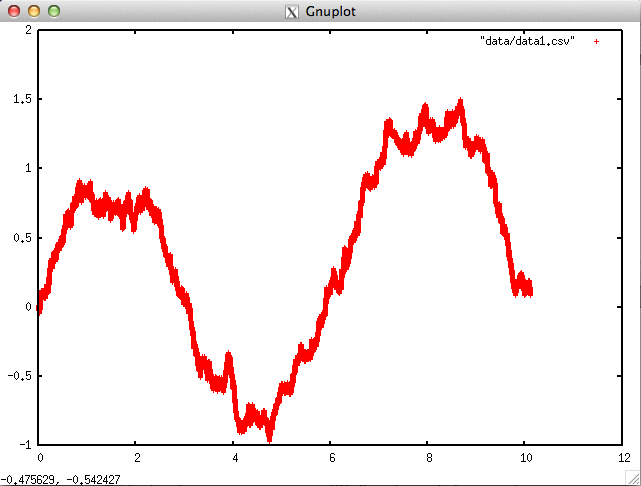
\includegraphics[width=0.6\textwidth]{gnuplot_interactive}      
  \end{center}
\end{frame}

\begin{frame}[fragile]{Vykreslení všech grafů v gnuplotu}
  \begin{verbatim}
    gnuplot> plot "data1.csv", "data2.csv", 
                  "data3.csv", "data4.csv"
  \end{verbatim}
  \pause
  \begin{center}
    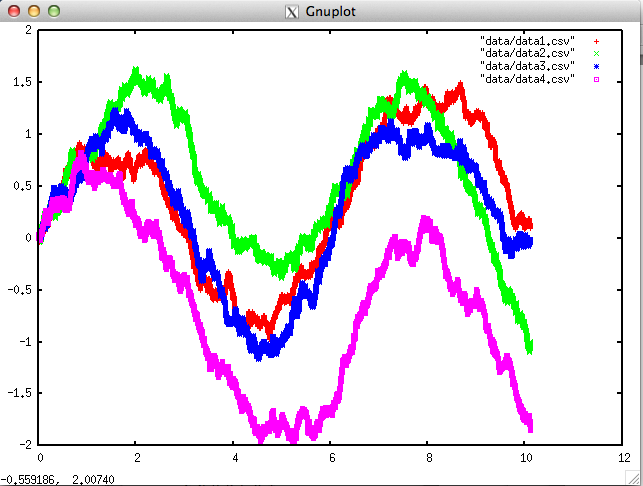
\includegraphics[width=0.6\textwidth]{gnuplot_interactive_all}  
  \end{center}
\end{frame}

\begin{frame}[fragile]{Dávkové použití}
  \scriptsize
  \begin{verbatim}
    set terminal png
    set output "plot4.png"
    plot "data/data1.csv", "data/data2.csv", \
         "data/data3.csv", "data/data4.csv"
  \end{verbatim}
  \pause 
  \begin{center}
    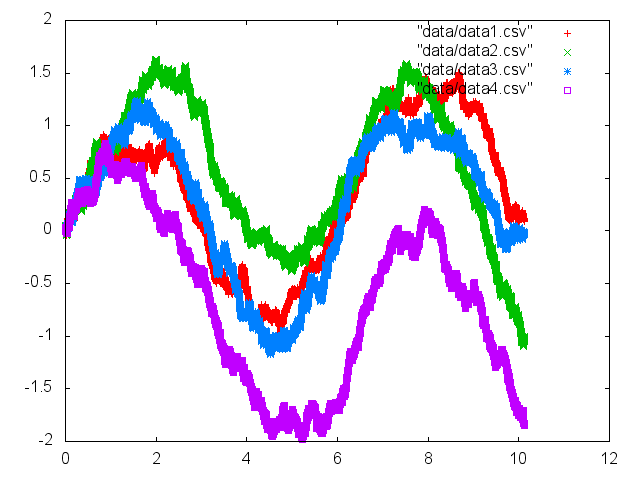
\includegraphics[width=0.6\textwidth]{../gnuplot/plot4}  
  \end{center}
\end{frame}

\begin{frame}[fragile]{BAT soubor}
  Je pracné pokaždé vypisovat parametry na příkazovou řádku. .BAT soubory ve Windows fungují jednoduše, prostě se do nich dá psát jako do terminálu a připravit si tak jednodušší skript.
  \begin{verbatim}
    gnuplot plot.gp
  \end{verbatim}
\end{frame}

\begin{frame}[fragile]{BAT soubor s parametrem}
  Co takhle adresář pro každý den? Nemá smysl pokaždé ručně kopírovat vstup pro gnuplot a tak dále... 
  
  Stačí vědět, že BAT soubor může mít na příkazové řádce parametry. První parametr je uložen do proměnné \texttt{\%1} a to se nám bude hodit.
  
  \begin{verbatim}
    cd %1
    gnuplot ../plot.gp
    cd ..
  \end{verbatim}
\end{frame}

\begin{frame}[fragile]{BAT soubor s parametrem - vylepšení}
  Pokud si budeme chtít prohlédnout grafy, bude nutné vždy vlézt do adresáře a otevřít \texttt{plot.png}. Jde to ovšem vylepšit pomocí jednoduchého triku:
  
  \begin{verbatim}
    cd %1
    gnuplot ../plot.gp
    copy plot.png ../%1.png
    cd ..
  \end{verbatim}
\end{frame}

\subsection{Zhodnocení}

\begin{frame}{Jak moc jsme si pomohli?}
  \begin{itemize}
    \item 
  \end{itemize}
\end{frame}

\subsection{Problém č. 2: jak na to?}

\begin{frame}{Stačí nám to na řešení problému č. 2?}
  Zatím nevíme, jak:
  \begin{itemize}
    \item vygenerovat vstupní soubory pro MCNP
    \item spustit hromadu MCNP výpočtů
    \item vytahat výsledky z MCNP výstupního souboru
  \end{itemize}
  Budeme potřebovat nějaký těžší kalibr.
\end{frame}

\section{Skriptovací jazyky}

\subsection{Úvod do skriptování}

\begin{frame}{``klasické'' programování -- Pascal, C++}
  
\end{frame}

\begin{frame}{Interpretované jazyky / skripty}
  
\end{frame}

\subsection{Úvod do jazyka Ruby}

\begin{frame}[fragile]{Ukázka Ruby (1)}
  Každý programátor tím začíná ...
  \begin{block}{}
    \smallskip \footnotesize
    \begin{verbatim}
      puts "Hello world!"
    \end{verbatim}    
  \end{block}
  \pause
  \begin{block}{}
    \smallskip \footnotesize
    \begin{verbatim}
      Hello world!
    \end{verbatim}
  \end{block}
\end{frame}

\begin{frame}[fragile]{Ukázka Ruby (2)}
  Proměnné, \texttt{print} vs. \texttt{puts}, aritmetika
  \begin{block}{}
    \smallskip \footnotesize
    \begin{verbatim}
      a = 4
      b = 5
      print "4 + 5 = "
      puts a + b
    \end{verbatim}    
  \end{block}
  \pause
  \begin{block}{}
    \smallskip \footnotesize
    \begin{verbatim}
      4 + 5 = 9
    \end{verbatim}
  \end{block}
\end{frame}

\begin{frame}[fragile]{Ukázka Ruby (3)}
  In-line výrazy v řetězcích
  \begin{block}{}
    \smallskip \footnotesize
    \begin{verbatim}
      a = 4
      b = 5
      puts "#{a} + #{b} = #{a+b}"
    \end{verbatim}    
  \end{block}
  \pause
  \begin{block}{}
    \smallskip \footnotesize
    \begin{verbatim}
      4 + 5 = 9
    \end{verbatim}
  \end{block}
\end{frame}

\begin{frame}[fragile]{Ukázka Ruby (4)}
  Rozsahy a cykly
  \begin{block}{}
    \smallskip \footnotesize
    \begin{verbatim}
      (1..5).each do |i|
        puts "#{i} * #{i} = #{i * i}"
      end
    \end{verbatim}    
  \end{block}
  \pause
  \begin{block}{}
    \smallskip \footnotesize
    \begin{verbatim}
      1 * 1 = 1
      2 * 2 = 4
      3 * 3 = 9
      4 * 4 = 16
      5 * 5 = 25
    \end{verbatim}
  \end{block}
\end{frame}


\begin{frame}[fragile]{Ukázka Ruby (4)}
  Pětkrát nic umořilo osla (opakování, ne cyklus)
  \begin{block}{}
    \smallskip \footnotesize
    \begin{verbatim}
      5.times do
        puts "nic"
      end
    \end{verbatim}    
  \end{block}
  \pause
  \begin{block}{}
    \smallskip \footnotesize
    \begin{verbatim}
      nic
      nic
      nic
      nic
      nic
    \end{verbatim}
  \end{block}
\end{frame}




\begin{frame}[fragile]{Určení poloh tyčí}
  \tiny
  \begin{verbatim}
    c ---------------------------------
    c polohy tyci (z-plochy)
    c ---------------------------------
    c
    67 pz 47.6000    $ dolni hranice absoberu r1
    68 pz 40.4980    $ dolni hranice hlavice r1
    69 pz 44.8000    $ dolni hranice absoberu r2
    70 pz 37.6980    $ dolni hranice hlavice r2
  \end{verbatim}
\end{frame}

\begin{frame}{A to je vše, přátelé!}
  \begin{center}
    
\includegraphics[width=\textwidth]{looney_tunes}
  \end{center}
\end{frame}

\end{document}
